A differenza dei casi precedenti, per i $\gamma$ i meccanismi sono totalmente differenti. Ciò perché i $\gamma$, essendo fotoni, sono privi di carica, per cui interagiscono con la materia in maniera diversa.

Nello spettro delle onde elettromagnetiche i raggi $\gamma$ sono le radiazioni più energetiche: corrispondono a energie che vanno da qualche centinaio di keV in su. Poiché nello spettro non c'è una vera e propria distinzione tra la zona dei $\gamma$ e le altre, oltre ai valori di energia bisogna ricordarsi che i fotoni $\gamma$ sono associati a processi legati al nucleo (ad esempio decadimenti $\gamma$ che riguardano le transizioni tra i livelli nucleari, mentre le transizioni tra livelli atomici comportano le emissioni di radiazioni ricadenti nella zona dei raggi $X$). Va ricordato che quanto diciamo riguardo l'interazione dei $\gamma$ è applicabile anche a quella dei raggi X.

Oltre le transizioni nucleari, altre sorgenti di raggi $\gamma$ (che peraltro portano a valori di energia più elevati) sono i $\gamma$ presenti nella radiazione cosmica e i $\gamma$ prodotti da collisioni tra fasci di particelle accelerate mediante acceleratori.

\section{Meccanismi di interazione dei fotoni}

I $\gamma$ sono delle radiazioni neutre ed i meccanismi di interazione che caratterizzano questi sono tipicamente catastrofici, nel senso che sono dei processi in cui il $\gamma$ perde una frazione consistente della propria energia, modificando profondamente lo stato iniziale, a differenza delle particelle cariche sia leggere che pesanti in cui l'interazione con la materia avviene gradualmente, attraverso processi multipli di interazione.

I meccanismi attraverso cui i $\gamma$ interagiscono con la materia sono essenzialmente tre:

\begin{itemize}
    \item Effetto fotoelettrico;
    \item Effetto Compton;
    \item Produzione di coppie $e^+ - e^-$.
\end{itemize}

Questa differenza nella modalità di interazione comporta due conseguenze: una prima conseguenza è che i raggi $X$ e $\gamma$ sono radiazioni molto più penetranti rispetto alle particelle cariche; la seconda è che fasci di questi raggi non si degradano in energia quando attraversano la materia, ma solo in intensità. Quindi se un $\gamma$ attraversa la materia ci sono solo due possibilità: o interagisce o non interagisce, per cui non accade, come nel caso delle particelle cariche, che attraversando uno spessore la particella perda parte della sua energia e poi fuoriesca dal materiale, bensì in questo caso o il $\gamma$ interagisce e scompare (perché cambia il suo stato e al suo posto si formano altri prodotti) oppure attraversa il materiale indisturbato; pertanto quando andiamo a studiare l'assorbimento dei $\gamma$ attraverso la materia osserviamo una diminuzione dell'intensità del fascio attraversante lo spessore, ma l'energia dei $\gamma$ fuoriuscenti sarà uguale a quella iniziale. Possiamo dunque dire che i fotoni che conservano il loro stato iniziale sono quelli che non hanno interagito.

A questo punto dobbiamo capire la probabilità con cui avviene ciascuno di questi processi di interazione. In generale si può dire che le sezioni d'urto d'interazione sono molto minori rispetto a quelle relative ai processi con particelle cariche. In altre parole, i fotoni interagiscono molto meno con la materia (ed è per questo che riescono ad attraversare grandi spessori di materiale, cioè hanno un potere penetrante molto più elevato) rispetto alle particelle cariche.

L'attenuazione dei fotoni incidenti in un dato materiale segue una legge di tipo esponenziale decrescente, simile a quella relativa alle particelle cariche leggere (elettroni e positroni), solo che in questo caso è una legge esatta mentre in quel caso era una legge semi-empirica derivante da vari fattori (le particelle non sono monocromatiche, si considera la convoluzione di tante curve di trasmissione ecc.).

L'intensità $I$ del fascio dopo aver attraversato uno spessore $x$ di materiale è data da

\begin{equation*}
    I=I_0 e^{-\mu x}
\end{equation*}

dove $I_0$ è l'intensità iniziale del fascio è $\mu$ è un coefficiente di assorbimento, che esprime la probabilità di interazione dei $\gamma$ per unità di percorso. Si può immaginare come una sorta di inverso del libero cammino medio del fotone all'interno della materia e dipende dal materiale, per cui si misura in $\rm cm^{-1}$ oppure in $\rm cm^2/g$.

Anche in questo caso è possibile possibile realizzare una curva di trasmissione, che ha in ascisse lo spessore attraversato e in ordinate il coefficiente di trasmissione $T=I/I_0$. Quello che otterremmo in questo caso sarebbe un esponenziale decrescente.

Ne approfittiamo per ricordare i vari andamenti:

\begin{itemize}
    \item Per particelle cariche pesanti abbiamo una curva a gradino smussato a causa degli effetti di straggling;
    \item Per particelle cariche leggere, se queste sono mono-energetiche la curva è a gradino ma molto smussato a causa dei percorsi molto frastagliati della particella nel materiale (straggling maggiore), se invece sono $\beta$ emessi da una sorgente, quindi con uno spettro di energia continuo, la curva è approssimabile con una legge esponenziale decrescente;
    \item Per i $\gamma$ la curva è proprio una legge esponenziale decrescente.
\end{itemize}

Il coefficiente di assorbimento $\mu$ si può esprimere anche con l'espressione

\begin{equation*}
    \mu=N \sigma_{\rm tot}
    =\frac{N_A \rho}{A} \sigma_{\rm tot}
\end{equation*}

dove si va moltiplicare la sezione d'urto di interazione totale (con cui includiamo tutti i possibili processi di interazione, dunque rappresenta la probabilità di interazione di un fotone con la materia indipendentemente dal tipo di processo) per la densità di atomi $N$. La stessa relazione può essere riscritta con il numero di Avogadro $N_A$, la densità $\rho$ è l'$A$ del materiale. Segue che maggiore è la probabilità di interazione, maggiore sarà $\mu$, perché significa che il $\gamma$ interagisce di più con la materia e quindi viene più facilmente assorbito.

\subsection{Sezione d'urto di interazione}

La sezione d'urto totale è data dalla somma di quelle relative ai tre processi principali:

\begin{equation*}
    \sigma_{\rm tot}
    =\sigma_{\rm phot} + Z \sigma_{\rm Comp} + \sigma_{\rm coppie}
\end{equation*}

dove la $\sigma_{\rm comp}$ viene moltiplicata per la $Z$ del materiale perché normalmente questa sezione d'urto viene espressa in unità di carica.

Poiché ciascuna di queste componenti è legata ad un processo diverso, esse avranno espressioni dipendenti dalle caratteristiche del materiale e dall'energia del fotone in maniere differenti.

\begin{esempio}
    In figura sono riportate le sezioni d'urto dei singoli processi al variare dell'energia del fotone, la quale va da $\rm 10^{-3} \; MeV (=1 \; keV)$ a $\rm 10^5 \; MeV (=100 \; GeV)$.\footnotemark \;La scala di entrambi gli assi è logaritmica, in modo da poter rappresentare numeri che variano in un intervallo molto ampio, in particolare per la sezione d'urto abbiamo un intervallo di 30 ordini di grandezza.

    \begin{figure}[H]
        \centering
        \includegraphics[width=\textwidth]{immagini/sezione_durto_interazione.png}
    \end{figure}
    
    Il contributo dell'effetto fotoelettrico è dato dalla linea fucsia, la quale ci dice che la probabilità che un fotone interagisca per effetto fotoelettrico diminuisce notevolmente all'aumentare dell'energia, per cui per energie più basse domina mentre per quelle più alte (dal GeV in su) è praticamente nulla.

    La linea blu rappresenta lo scattering Compton incoerente, quella arancione quello coerente. Lo scattering coerente si ha quando l'elettrone non fuoriesce dall'atomo, cioè non viene strappato da questo, quello incoerente quando l'elettrone con cui il $\gamma$ interagisce fuoriesce. La curva blu sale per poi scendere, quella arancione non ha salite e diminuisce molto di più. La somma di questi due contributi dà la sezione d'urto dello scattering Compton, che dà una curva che tende leggermente a salire per poi diminuire a più elevate energie ed è una curva che prevale ad energie intermedie.

    Infine le linee azzurre, una continua e una tratteggiata, sono relative al contributo della produzione di coppie. Ce ne sono due perché la produzione di coppie si verifica sempre in presenza di un terzo corpo, che può essere un nucleo o un elettrone, per cui si hanno due casi diversi (la sezione d'urto maggiore è relativa al caso del nucleo). Tale contributo è nullo al di sotto del valore di soglia di 1.022 MeV, dopodiché aumenta fino a diventare il contributo più importante per le energie più elevate.

    Il grafico a sinistra è relativo all'alluminio. Se andiamo a materiali più pesanti come il piombo (grafico a destra) i valori cambiano, ma persistono le considerazioni appena fatte; ciò che invece è più evidente sono le strutture, nella sezione d'urto dell'effetto fotoelettrico, legate alle transizioni atomiche, quindi il valore di energia del fotone che sta incidendo sugli atomi di quel materiale corrisponde esattamente all'energia di una transizione atomica, per cui si vanno a vedere dei picchi.
\end{esempio}

\footnotetext{Per valori che vanno da $10^{-3}$ a $10^{-2}$ MeV si parla di raggi $X$, oltre sono $\gamma$.}

\subsection{Coefficiente di assorbimento}

\begin{esempio}
    In figura è riportato il coefficiente di assorbimento totale per il rame in funzione dell'energia. Esso è riportato in unità di densità superficiale, di modo che le curve ottenute al variare del materiale siano tra loro confrontabili.
    \begin{figure}[H]
        \centering
        \includegraphics[width=8cm]{immagini/coefficiente_assorbimento_gamma_rame.png}
    \end{figure}
    Per come è definito $\sigma_{\rm tot}$ (ricordiamo che $\mu$ è proporzionale a quest'ultimo), esso avrà un andamento che rispecchia l'andamento della somma delle tre sezioni d'urto. All'aumentare dell'energia $\mu$ diminuisce, per cui se abbiamo dei fotoni di energia molto elevata la probabilità che essi interagiscono con la materia diventa estremamente rara.
    
    Notiamo che nel grafico figurano due linee: la linea continua rappresenta il coefficiente di assorbimento, mentre quella tratteggiata rappresenta il "coefficiente di assorbimento massa-energia", il quale rappresenta la frazione media di particelle cariche prodotte dall'interazione dei gamma con la materia. Infatti tutti e tre i meccanismi di interazione portano alla produzione, nello stato finale, di particelle cariche, e andando a valutare quante ne vengono prodotte si può rappresentare il numero di queste in funzione dell'energia. Ciò che ci aspettiamo è che se i $\gamma$ interagiscono parecchio vengono prodotte tante particelle cariche, dunque anche questo numero è particolarmente elevato; man mano che l'energia aumenta questo numero tende a diminuire perché i $\gamma$ interagiscono di meno. La differenza tra le due curve sta nel fatto che intervengono tutti e tre i processi e ognuno di questi produce un numero di particelle cariche diverso, quindi dipende da qual è l'effetto dominante nella zona di energia in cui ci troviamo.
\end{esempio}

\begin{approfondimento}[Coefficiente di attenuazione e coefficiente di assorbimento]
    \footnotesize Attenzione! Questa nota è stata realizzata unendo quando detto da chatgpt e quanto trovato in "Introduction to Health Physics" di Herman Cember e Thomas E. Johnson. Il lettore attento noterà la discrepanza con quanto affermato dalla professoressa, per cui non garantisco la correttezza delle informazioni riportate.
    
    Approfondiamo il concetto di coefficiente di assorbimento. Diciamo innanzitutto che talvolta nei testi viene chiamato coefficiente di attenuazione, che può essere distinto tra linear attenuation coefficient ($\mu_l$) se espresso in $\rm cm^{-1}$ e mass attenuation coefficient ($\mu_m$) se diviso per la massa e dunque espresso in $\rm cm^2/g$:
    \begin{equation*}
        \mu_{m}=\frac{\mu_l}{\rho}
    \end{equation*}
    Come abbiamo già detto, esso è l'inverso del libero cammino medio. Quest'ultimo il Knoll lo chiama $\lambda$ e lo definisce come
    \begin{equation*}
        \lambda
        =\frac{\int_{0}^{+\infty} xe^{-\mu x} \dd{x}}{\int_{0}^{+\infty} e^{-\mu x} \dd{x}}
        =\frac{1}{\mu}
    \end{equation*}
    Il coefficiente di attenuazione dà la probabilità di rimozione di un fotone dal fascio ad opera di uno dei possibili meccanismi di interazione. Il coefficiente di attenuazione totale, dunque, è dato dalla somma dei coefficienti per ciascuno dei tre processi:
    \begin{equation*}
        \mu=\mu_{\rm phot} + \mu_{\rm Comp} + \mu_{\rm coppie}
    \end{equation*}
    Tale equazione dà la frazione di energia rimossa dal fascio per unità di spessore attraversato. La frazione di energia del fascio che viene depositata nell'assorbitore considera però soltanto l'energia trasferita al materiale dai fotoelettroni, dagli elettroni Compton e dalle coppie $e^+ - e^-$, mentre l'energia trasportata via dal fotone scatterato per effetto Compton e quella portata via dalla radiazione ottenuta per annichilazione di coppie non vengono tenute in conto. Il coefficiente di assorbimento energia, detto anche vero coefficiente di assorbimento, è dato da
    \begin{equation*}
        \mu_{\rm en}
        =\mu_{\rm phot} + \mu_{\rm Comp} + \mu_{\rm coppie} \qty( \frac{h \nu - 1.02}{h\nu} )
    \end{equation*}
    Ovviamente, il coefficiente di assorbimento massa energia si otterrà semplicemente dividendo questo per la densità del materiale.

    \begin{minipage}{0.495\textwidth}
        \begin{figure}[H]
            \centering
            \includegraphics[width=0.8\textwidth]{immagini/coefficiente_assorbimento_vs_attenuazione.png}
        \end{figure}
    \end{minipage}
    \begin{minipage}{0.5\textwidth}
        In sintesi, mentre il coefficiente di assorbimento ($\mu$) riguarda la probabilità di qualsiasi tipo di interazione del fotone gamma con la materia, il coefficiente di assorbimento massa energia ($\mu_{\rm en}$) si focalizza sull'energia effettivamente assorbita e trasferita alla materia, un aspetto cruciale per determinare gli effetti biologici delle radiazioni. In figura a lato possiamo vedere l'andamento dei due termini.
    \end{minipage}

    \vspace{0.2cm}In altri termini ancora, il coefficiente di attenuazione quantifica la riduzione dell'intensità del fascio, mentre il (vero) coefficiente di assorbimento quantifica la frazione di energia assorbita dal fascio, entrambi per unità di spessore di materiale attraversato. Entrambi dipendono dall'energia del fotone e dal materiale.
\end{approfondimento}

Richiamiamo adesso brevemente i tre processi presi in esame.

\subsection{Effetto fotoelettrico}

Esso si verifica solo nel caso di elettroni legati, in quanto un elettrone libero non potrebbe mai assorbire un fotone e assicurare la conservazione dell'impulso, quindi è necessaria la presenza di un nucleo che assorba l'impulso di rinculo.

L'effetto fotoelettrico consiste nel fatto che un fotone (cioè un $\gamma$) venga assorbito totalmente e un elettrone venga emesso dall'atomo, per cui alla fine si ha un elettrone più uno ione:

\begin{figure}[H]
    \centering
    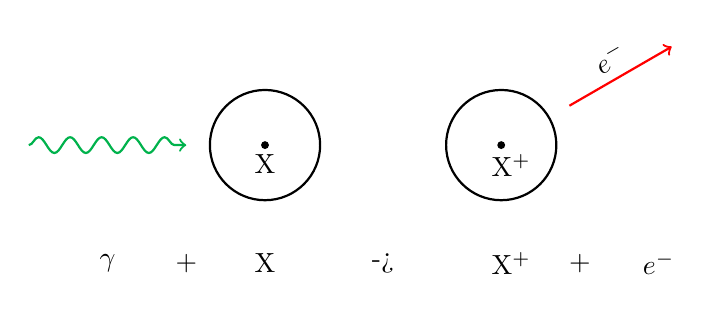
\begin{tikzpicture}
        %figura a sinistra
        \draw[->,thick, teal!60!green, decorate, decoration={snake, segment length=4mm, amplitude=1mm,post length=1mm}] (0,0) -- (2,0);
        \node at (1,-1.5) {$\gamma$};
        \node at (2,-1.5) {$+$};
        \filldraw (3,0) circle (1.2pt) node[below] {X};
        \draw[thick] (3,0) circle (0.7cm);
        \node at (3,-1.5) {X};
        \node at (4.5,-1.5) {\ce{->}};
        %figura a destra
        \draw[->, thick, red,rotate around={30:(6,0)}] (7,0) -- (8.5,0) node[midway, above, rotate=30, black] {$e^-$};
        \filldraw (6,0) circle (1.2pt) node[below] {\hspace{0.25cm}X$^+$};
        \draw[thick] (6,0) circle (0.7cm);
        \node at (6,-1.5) {$\hspace{0.25cm}\rm X^+$};
        \node at (7,-1.5) {$+$};
        \node at (8,-1.5) {$e^-$};
    \end{tikzpicture}
\end{figure}

Affinché ciò avvenga, è necessario che l'energia del fotone incidente superi un certo valore di soglia $W_0$, che è il lavoro di estrazione. In altre parole, il fotone incidente di energia $h\nu$ deve avere un'energia tale da strappare l'elettrone all'atomo, il quale verrà emesso con un'energia cinetica data dalla relazione:

\begin{equation*}
    K_{\rm max}=h\nu - W_0
\end{equation*}

$W_0$ è dell'ordine di pochi eV ma dipende dal materiale.

Essendo i $\gamma$ fotoni ad altissima energia siamo certamente al di sopra del lavoro di estrazione degli elettroni di un qualsiasi materiale, inoltre in questo caso possiamo dire che l'energia cinetica $K_{\rm max}$ dell'elettrone espulso dall'atomo può essere approssimata all'energia del fotone incidente\footnote{Infatti per dare un'idea delle quantità in gioco possiamo immaginare di avere un $\gamma$ di energia 1 MeV che incide su un materiale avente lavoro di estrazione pari a 2 eV: il fotoelettrone emesso avrà energia pari a $(10^6 - 2)$ eV, che è praticamente una differenza irrisoria.}. Di conseguenza, nel caso delle sorgenti $\gamma$ che adopereremo in laboratorio varrà questa approssimazione, cioè potremo dire che gli elettroni emessi per effetto fotoelettrico hanno energia praticamente identica a quella del $\gamma$ incidente.

Ribadiamo che non sempre è così: se andiamo verso radiazioni a più basse energie la differenza non è più trascurabile, seppur si riesca comunque a produrre effetto fotoelettrico (ad esempio la luce visibile può produrre effetto fotoelettrico su alcuni materiali, così come vedremo utilizzando dei led per misurare la costante di Planck).

\begin{minipage}{0.395\textwidth}
    \begin{figure}[H]
        \centering
        \includegraphics[width=0.9\textwidth]{immagini/sezione_durto_effetto_fotoelettrico.png}
    \end{figure}
\end{minipage}
\begin{minipage}{0.6\textwidth}
    La sezione d'urto per effetto fotoelettrico dipende dal materiale e dall'energia della radiazione $\gamma$ incidente mediante una relazione del tipo

    \begin{equation*}
        \sigma_{\rm phot} \approx \frac{Z^5}{E_{\gamma}^{7/2}}
    \end{equation*}

    Ne segue che per agevolare l'effetto fotoelettrico conviene considerare materiali via via più pesanti, a $Z$ maggiore, mentre la dipendenza dall'energia del $\gamma$ spiega la brusca diminuzione di $\sigma$ vista nei grafici.
\end{minipage}

\vspace{0.3cm}In realtà tale dipendenza da $Z$ è valida solo per un certo intervallo di energie. Ad esempio a basse energie viene modificata. Il motivo è che valutare la sezione d'urto di questo processo non è semplice a causa della complessità delle funzioni d'onda degli elettroni negli atomi. Questa dipendenza dunque si presenta per energie al di sopra della shell K (livello 1s), a circa $10^{-1}$ MeV, per valori più bassi cambia forma\footnote{Ti aspettavi un approfondimento a questo punto? Non stavolta! Servono concetti di AQM e qui siamo solo alla triennale, non bruciamo le tappe.}.

Nella figura sopra possiamo vedere l'andamento della sezione d'urto per effetto fotoelettrico nel caso del piombo. Notiamo come la parte iniziale è caratterizzata dalle transizioni atomiche. Ricordiamo che esso governa l'interazione a basse energie.

\subsection{Effetto Compton}

\E un effetto di scattering di un fotone su un elettrone.

\begin{figure}[H]
    \centering
    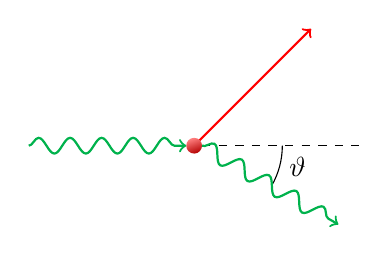
\begin{tikzpicture}
        %elettrone
        \draw[thick,->,red,rotate around={45:(2.1,0)}] (2.1,0) -- (4.2,0); 
        \shade[top color=red!50,bottom color=red!70!black,shading angle=20] (2.1,0) circle (0.1cm);
        %fotone incidente
        \draw[->,thick, teal!60!green, decorate, decoration={snake, segment length=4mm, amplitude=1mm,post length=1mm}] (0,0) -- (2,0);
        %angolo
        \draw[dashed] (2.2,0) -- (4.2,0);
        \draw (3.22,0) arc (0:-30:1.02cm) node[midway, right] {$\vartheta$};
        %fotone riflesso
        \draw[->,thick, teal!60!green, decorate, decoration={snake, segment length=4mm, amplitude=1mm,post length=1mm},rotate around={-30:(2.2,0)}] (2.2,0) -- (4.2,0);
      \end{tikzpicture}
\end{figure}

In questo caso si considera l'effetto su un elettrone libero. In realtà gli elettroni sono quelli atomici, però si può considerare un elettrone atomico come libero per il fatto che le energie di legame degli elettroni sono normalmente molto più piccole rispetto alle energie dei $\gamma$ considerati, quindi è un'approssimazione lecita. 

A seguito dello scattering, nello stato finale avremo un fotone diffuso, con energia $h\nu'$ inferiore rispetto all'energia $h\nu$ del fotone incidente, e un elettrone.

Indicando con $\vartheta$ l'angolo di diffusione del fotone uscente, applicando la conservazione dell'energia e dell'impulso è possibile individuare una relazione che lega l'energia del fotone diffuso con l'angolo:
\begin{equation*}
    h\nu'=\frac{h\nu}{\big[1 + \gamma (1 - \cos{\vartheta})\big]}
    \qqtext{dove}
    \gamma=\frac{h\nu}{m_ec^2}
\end{equation*}
Quindi in base al valore di $\vartheta$, che varia da evento a evento, le energie ripartite tra l'elettrone e il fotone diffuso possono essere differenti.
Per la conservazione dell'energia, l'energia cinetica dell'elettrone sarà data dalla differenza tra l'energia del fotone incidente e quello diffuso:
\begin{equation*}
    T_e=h\nu - h\nu'
\end{equation*}
Tale processo domina a energie intermedie.

Lo scattering Compton si definisce coerente quando l'elettrone, che consideriamo libero ma in realtà non lo è, rimane legato all'atomo; se invece l'elettrone acquisisce un'energia tale da poter essere strappato dall'atomo si parla di scattering incoerente. Più precisamente:

\begin{itemize}
    \item Lo scattering coerente (anche noto come scattering di Rayleigh) si verifica quando il fotone è deviato dalla sua traiettoria originale senza perdita di energia. In questo caso, l'interazione è elastica e avviene principalmente con l'intero atomo piuttosto che con singoli elettroni. Anche se lo scattering coerente non modifica l'energia del fotone, può comunque contribuire alla diffusione della radiazione;
    \item Lo scattering incoerente, che si riferisce specificamente allo scattering Compton, si verifica quando il fotone cede parte della sua energia a un elettrone e viene diffuso con una lunghezza d'onda maggiore. Questa interazione è inelastica e comporta un cambiamento nella lunghezza d'onda del fotone.
\end{itemize}

La sezione d'urto Compton è data da due termini che corrispondono a quello coerente e a a quello incoerente\footnote{Questa affermazione è parzialmente in contrasto con quanto detto subito dopo. Non è sbagliato dire che i due contributi sono questi, ma quelli mostrati nel grafico sono altri due.}. Si osserva una dipendenza lineare da $Z$, e una diminuzione che ad alte energie può essere parametrizzata con una dipendenza del tipo $(\ln E)/E$.

\begin{minipage}{0.375\textwidth}
    \begin{figure}[H]
        \centering
        \includegraphics[width=\textwidth]{immagini/sezione_durto_effetto_Compton.png}
    \end{figure}
\end{minipage}
\begin{minipage}{0.62\textwidth}
    Due quantità utili che possono essere calcolate tramite la formulazione di Klein-Nishina sono le sezioni d'urto di scattering Compton e di assorbimento Compton. La sezione d'urto di scattering Compton, $\sigma_{\rm s}$, è definita come la frazione media dell'energia totale contenuta nel fotone diffuso, mentre la sezione d'urto di assorbimento, $\sigma_{\rm a}$, è l'energia media trasferita all'elettrone di rinculo. Poiché l'elettrone è fermato dal materiale, questa è la frazione media di energia assorbita dal materiale nello scattering Compton. Ovviamente si ha
\end{minipage}

\begin{equation*}
    \sigma_{\rm Comp}=\sigma_{\rm a} + \sigma_{\rm s}
\end{equation*}

Attenzione! Rispetto ai grafici precedenti in questo sembra che tale contributo decresca più velocemente, ma ciò è dovuto semplicemente al fatto che stiamo considerando un intervallo più ristretto di energie.

\subsection{Creazione di coppie}

Con questo processo si ha una creazione di una coppia elettrone-positrone a partire da un $\gamma$. Ciò può avvenire solo in presenza di un terzo corpo per questioni di conservazione dell'impulso.

\begin{figure}[H]
    \centering
    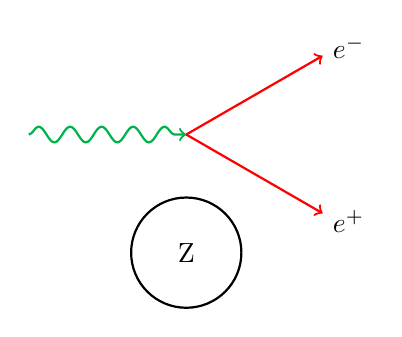
\begin{tikzpicture}
        \draw[thick,->,red,rotate around={30:(2,0)}] (2,0) -- (4,0) node[above=.1cm, right, black] {$e^-$};
        \draw[thick,->,red,rotate around={-30:(2,0)}] (2,0) -- (4,0) node[below=.1cm, right, black] {$e^+$};
        %fotone incidente
        \draw[->,thick, teal!60!green, decorate, decoration={snake, segment length=4mm, amplitude=1mm,post length=1mm}] (0,0) -- (2,0);
        \draw[thick] (2,-1.5) node {Z} circle (0.7cm);
      \end{tikzpicture}
\end{figure}

Questo terzo corpo tipicamente è il nucleo atomico, ma alcune volte tale processo può avvenire anche nel campo degli elettroni, infatti nel grafico della sezione d'urto c'erano due termini relativi alla produzione di coppie, ma quello relativo al caso dell'elettrone è trascurabile rispetto all'altro.

La coppia prodotta deve rispettare la conservazione dell'energia, per cui l'energia cinetica delle due particelle uscenti corrisponde all'energia del fotone incidente meno due volte la massa a riposo dell'elettrone:

\begin{equation*}
    T(e^+) + T(e^-)=h\nu - 2mc^2
\end{equation*}

Ciò ha senso, perché parte dell'energia del fotone deve essere usata per la produzione delle due masse.

\begin{minipage}{0.395\textwidth}
    \begin{figure}[H]
        \centering
        \includegraphics[width=5cm]{immagini/sezione_durto_produzione_coppie.png}
    \end{figure}
\end{minipage}
\begin{minipage}{0.6\textwidth}
    Da tale relazione segue che ci sia una soglia di produzione al di sotto della quale è impossibile che si verifichi il processo di produzione di coppie. Quindi, se il fotone incidente non ha un'energia sufficiente almeno a creare questa coppia (cioè almeno $2mc^2=1.022$ MeV), non avviene nessun processo; se ha un'energia superiore alla soglia, quella in eccesso viene poi suddivisa tra i prodotti, cioè tra elettrone e positrone.

    La sezione d'urto è proporzionale a $Z^2$ e cresce con l'energia, infatti è il processo che domina ad energie elevate.
\end{minipage}

\vspace{0.2cm}In figura possiamo vedere l'andamento della sezione d'urto per produzione di coppie in funzione dell'energia nel caso del piombo. Notiamo come essa sia nulla al di sotto del valore di soglia.

\subsection{Sommario}

\begin{itemize}
    \item A bassa energia (ordine del MeV) i fotoni interagiscono prevalentemente mediante effetto fotoelettrico, che produce un elettrone avente pressoché la stessa energia del $\gamma$;

    \item Per energie tra 1 e 10 MeV prevale l'effetto Compton, che produce un elettrone ed un fotone diffuso che si dividono l'energia del fotone iniziale;
    \item Ad alte energie (sopra i 10 MeV) prevale il processo di produzione di coppie, che nello stato finale produce una coppia $e^+ - e^-$.
\end{itemize}

\comment{
\section{Sciami elettromagnetici}

Ci chiediamo adesso come interagiscono questi prodotti secondari (elettroni, positroni, fotoni) con la materia. Infatti, se in partenza abbiamo elettroni o fotoni di energia particolarmente elevata, si innesca un meccanismo di produzione a valanga, nel senso che si produce una \textbf{cascata elettromagnetica} (o sciame e.m.), che è una sequenza di processi di bremsstrahlung e di produzione di coppie che porta alla produzione di un insieme di particelle ($e^+, e^-$, fotoni) che man mano si propagano nella materia.


Immaginiamo di avere ad esempio inizialmente un fotone particolarmente energetico che incide su un materiale assorbitore. Avendo energia elevata, a un certo punto darà luogo ad un processo di produzione di coppie $e^+ - e^-$. Ciascuno di questi sarà ad alta energia, per cui per dare una parte di questa attraverso bremsstrahlung, quindi la sequenza continua con un fotone di Brahms 3 lunga il positrone/elettrone di partenza che a loro volta daranno luogo ad altri processi che saranno produzioni di coppie o ulteriori processi di bremsstrahlung. Quindi da un singolo fotone incidente di alta energia si produce uno sciame elettromagnetico, composto da un numero di particelle via via crescente.

Uno sciame elettromagnetico può essere indotto, oltre che da un fotone ad alta energia, anche da un elettrone può si trovano ad alta energia, solo che il primo processo sarà di bremsstrahlung e non di produzione di copie. Esso viene detto elettromagnetico perché è uno scemo in cui vengono coinvolti solo processi elettromagnetici punto è composto da $ e^+,e^-$ e $\gamma$ (fotoni) e si differenzia da uno sciame adronico, che indotto da adroni ad alta energia e in cui vi sono processi e coinvolgono l'interazione forte. Tuttavia tali sciami potrebbero avere al loro interno anche una componente elettromagnetica, legata alla possibile produzione di Pioli neutri "cadono in due $\gamma$ Che poi saranno luogo a questa componente.

Man mano che lo sciame si propaga all'interno del materiale, continuano a verificarsi processi di breve straming e produzione di coppie. Questo meccanismo ovvero non procede all'infinito, perché a un certo punto l'energia dei prodotti secondari diminuiranno, in quanto l'energia iniziale si suddividerà tra un numero di particelle di via crescente, arrivando sotto il valore di energia critica (energia in corrispondenza della quale la sezione d'urto per perdita di energia collisionale è la stessa di quella per perdita di energia radiativa, C'è qui la probabilità è la stessa). Quando gli elettroni raggiungono questo valore, non interagiscono con la materia soltanto attraverso fenomeni di bremsstrahlung ma possono subire anche altri fenomeni collisionali, in cui non vengono prodotte nuove particelle punto per quanto riguarda i fotoni, man mano che la loro energia diminuisce non daranno luogo a produzioni di coppie, ma cominceranno a prevalere altri effetti, come quello fotoelettriche e quello Compton punto in conseguenza ciò non possiamo dire che lo sciame si arresti perché le particelle continueranno a provocarsi all'interno del materiale finché non perdono tutta la loro energia, però possiamo dire che il numero di particelle dello sciame non aumenterà superato il punto critico. Al di sotto dell'energia critica possiamo quindi immaginare che lo sciame che man mano è cresciuto (sia in dimensioni che nel numero di particelle), incomincia a degradarsi, pertanto il numero di particelle comincia a diminuire perché esse continuano a interagire, perdendo energia e venendo assorbite totalmente dal materiale.

Proviamo ora a immaginare un modello semplificato per descrivere la struttura di uno sciame elettromagnetico. Esso si basa sul concetto di lunghezza di radiazione, in quanto la distanza percorsa viene espressa in multipli di lunghezza di radiazione. Inoltre immaginiamo che in corrispondenza di ogni lunghezza di radiazione si verifichi in media un nuovo processo che può essere di produzione di coppie di bremsstrahlung. Si definisce quindi il numero di generazione, dato al rapporto tra lo spazio percorso e la lunghezza di radiazione:

\begin{equation*}
    t=\frac{x}{x_0}
\end{equation*}

\begin{equation*}
    \frac{E}{2^t}=E_C
    \implies
    t=\frac{\ln{E/E_C}}{\ln{2}}
\end{equation*}

utilizzando delle opportuni variabili, anche studiandole con dei modelli molto semplici, lo shame adronico invece è qualcosa di estremamente complesso. Quindi noi ci limiteremo allo studio di questi sciami rettromagnetici. Come prosegue lo shame? Abbiamo capito che, man mano che si propaga all'interno del materiale, continuano a verificarsi in successione questi fenomeni di brainstorm e di creazione di coppie. Tuttavia questo meccanismo non procede all'infinito, perché è arrivato a un un punto le energie dei prodotti secondari, man mano diminuiranno perché capite partite da un unico fotone o elettrone di alta energia e man mano che si producono le particelle, l'energia ovviamente viene suddivisa tra i diversi prodotti delle particelle. Quindi man mano l'energia si degrada, va a diminuire fino a quando gli elettroni avranno una energia che sarà all'isotto dell'energia critica che abbiamo definito la volta scorsa. Se Se ricordate l'energia critica era l'energia in corrispondenza della quale la sezione d'urto per perdita di energia condizionale è la stessa, viene guagliata dalla sezione d'urto di perdita di energia radiativa, quindi quindi un valore di energia in corrispondenza del quale c'è la stessa probabilità che l'elettrone perde energia perfetti condizionali e perfetti radiativi. Quindi quando si raggiunge questo valore di energia critica, capitate gli elettroni a questo punto non interagiscono con la materia soltanto attraverso fenomeni di Bremstra, a a ma possono subire anche fenomeni condizionali, quindi perdere energia attraverso altri meccanismi e ovviamente nei fenomeni condizionali non vengono prodotte delle nuove particelle come avveniva nel caso delle Bremstra, in cui veniva emesso un nuovo fotone. A sua volta i fotoni, man mano che diminuiscono, man mano che si propagano nel materiale, quindi diminuiscono la loro energia, non deranno più luogo poi a fenomeni di produzione di coppie ma incominceranno a prevalere altri effetti come l'effetto fotelettrico e l'effetto Comton. Quindi si arriverà sostanzialmente a un punto in corrispondenza del quale gli elettroni procederanno a perdere la propria energia attraverso processi condizionali. I fotoni cominceranno a interagire attraverso meccanismi di Schettering-Comton ed effetto fotelettrico e di conseguenza lo Sjame non possiamo dire che si arresta, perché lo Sjame non si ferma, quindi quindi particelle prodotte continueranno a propagarsi all'interno del materiale, anche non perdono tutta la loro energia. Però certamente non aumenterà in termini di numero di particelle, perché abbiamo detto appunto non verranno più prodotti dei nuovi fotoni di Bremstra-Lung e non vengono più prodotte neanche coppie e più e meno. Quindi al massimo ad esempio un elettrone darà luogo un effetto fotelettrico, quindi quindi che avevo un fotone mi ritropevo un sole elettrone, capite che non aumenta più il numero di particelle che compongono lo Sjame elettromagnetico. Al di sotto dell'energia critica, quindi quindi posso immaginare che lo Sjame che Mammano e Cresciuto sia in dimensioni che il numero di particelle incomincia a degradarsi e quindi innanzitutto il numero di particelle comincia a diminuire perché le particelle Mammano continuano a interagire a perdere energia e a essere totalmente assorbite del materiale. Possiamo provare a immaginare un modello semplificato per descrivere la struttura di uno Sjame elettromagnetico e questo modello si basa sostanzialmente sul concetto di lunghezza di radiazione che abbiamo visto la volta scorsa, una grandezza caratteristica del materiale. Quindi ora noi lavoreremo esprimendo la distanza percorsa in molti di lunghezza di radiazione. Io posso immaginare che in corrispondenza di ogni lunghezza di radiazione si verifichi in media un nuovo processo che può essere o un processo di produzione di coppie o un processo di Bremstra-Lung. E allora vado a definire T come il numero di generazioni, quindi sostanzialmente il rapporto tra lo spazio percorso e questa lunghezza di radiazione. Quindi quante lunghezze di 

radiazioni sono state percorse fino ad esso questo numero è espresso proprio da T. Guardiamo schematicamente l'immagine che ci ritroviamo a destra. Sostanzialmente abbiamo in partenza un ad esempio un $\gamma$ di alta energia che interagisce quindi, produce una coppia $e^+ - e^-$. Questa coppia percorre uno spazio che all'incirca è appunto una lunghezza di radiazione e poi dal luogo a Bremstra-Lung. Nel Bremstra-Lung viene prodotto un fotone e un elettrone come stato finale. La stessa cosa quindi per il positrone e dopo una lunghezza di radiazione, normalmente normalmente fotone produrrà a coppia, l'elettrone produrrà a Brestralong e la stessa cosa per l'altro ramo che abbiamo qui sulla destra. Quindi cosa notiamo? che, indipendentemente dalla particella che vado a considerare che sia un fotone o un elettrone o un positrone, a me quello che interessa è che ogni volta che percorro uno spazio pare una lunghezza di radiazione, quello che succede è che ogni particella si raddoppia. Quindi se ad esempio guardiamo la prima interazione da una particella passiamo a 2, poi da 2 particelle passiamo a 4, poi da 4 passiamo a 8 e così via. Insomma ogni volta il numero di particelle si moltiplica di un fattore 2. Quindi possiamo generalizzare questo meccanismo andando a dire che il numero di particelle prodotte dopo t lunghezza di radiazione sarebd appare a 2 in alzata t. Stiamo d'accordo quindi ad esempio t u e la 3, 2 in alzata 3, 8 e sono effettivamente 8 particelle. Ora quale sarà l'energia di queste particelle? L'abbiamo detto ma a mano l'energia si degrada perché l'energia del fotone incidente viene via via suddivisa nei prodotti di questa cascata e quindi posso dire che che che andrà a dire che queste ad esempio 8 particelle che mi ritrovo a questo livello 3, quindi dopo 3 lunghezze di radiazione, abbiano in media un'energia che pari all'energia del fotone incidente diviso 8. Quindi anche in questo caso generalizzando posso dire che in media una particella prodotta alla t'esima lunghezza di radiazione corrisponde all'energia incidente diviso il numero di particelle prodotte, quindi 2 in alzata t. E allora se partiamo da questa relazione posso andare a valutare quante particelle ad esempio venono prodotte in corrispondenza dell'energia critica perché vi ho detto che lo shame aumenta in numero quindi aumentano le particelle che compongono lo shame fin quando non si raggiunge questa famosa energia critica al di sotto della quale poi prevalgono altri meccanismi come il processo collizionale per gli elettroni e l'effetto fotoelettrico, l'effetto Compton per i $\gamma$ per cui lo shame non aumenta più in numero come numero di particelle. Quindi posso immaginare che il massimo dello shame inteso come massimo numero di particelle venga raggiunto in corrispondenza dell'energia critica. E allora se vado a igualliare l'energia media che è ogni singola particella alla generazione t a questo valore di energia critica quindi sostanzialmente prendo questo valore e di t che pari a e diviso 2 alla t e l'o uaglio e l'energia critica allora sostanzialmente mi sto analizzando la situazione in cui sono arrivata l'energia critica e lo shame non si sviluppo ulteriormente. Dopo quanto abbiamo, quanto spazio ha percorso il mio shame fino a raggiungere questa condizione allora basta che valuto quante lunghezze di radiazioni sono state percorse quindi ricavo da questa equazione il valore di t. Allora con dei semplici passaggi 

potete andare a scrivere che è diviso l'energia critica e pari a 2 in alza di t ed è qui ricavare il valore di t e vedete che t si esprime come il logaritmo di e sui concì diviso logaritmo di 2 che ovviamente un valore costante. Di questa relazione che vi ho evidenziato in arancione ci interessa in particolare la dipendenza dall'energia quindi sto dicendo che ho uno shame che si sta man mano propagando e sta aumentando il numero di particelle e questo shame si propaga ma ha arrivato a un certo punto dopo aver percorso un certo numero di lunghezze di radiazione l'energia delle particelle prodotte è così bassa che ha raggiunto il valore di energia critica e di conseguenza lo shame non si sviluppo ulteriormente ha raggiunto il massimo numero di particelle. Dori in avanti quindi quello che mi aspetta è che man mano poi questo shame incomincia a degradarsi cioè queste particelle man mano vengono assorbite dal materiale ma se sono interessata al punto in cui chi raggiunge questo massimo numero di particelle allora questo valore dipende con una relazione logaritmica dall'energia incidente quindi dall'energia del fotone o dell'elettrone iniziale e perché è interessante questa relazione perché ad esempio volete immaginare di individuare quanto spessore di un dato materiale è necessario per poter arrestare o contenere comunque lo shame di una data energia ok perché importante perché ad esempio dal punto di vista della rivelazione esistono dei rivelatori che prendere il nome di calorimetri questi sono dei rivelatori che come richiamano la stessa nome sono progettati per andare a misurare tutta l'energia di una particelle incidente quindi se ad esempio io volessi andare a misurare dei $\gamma$ o degli elettroni molto energetici e utilizzo un rivelatore quello che succederà quando questo $\gamma$ o questo elettrone entra nel mio rivelatore sarà la produzione di uno shame perché questo quello che avviene in qualsiasi materiale e allora per misurare tutta l'energia dell'oshame io mi devo assicurare che tutte le particelle prodotte nell'oshame rimangano all'interno del rivelatore quindi il rivelatore non può essere troppo corto perché quello che può succedere è che che in comincia a propagarsi ma poi fuoriesce dal materiale e quindi perdo parte dell'oshame quindi parte dell'energia quindi è importante che la dimensione del rivelatore sia dimensionata alla dimensione dell'oshame che si può produrre e quindi mi domando che spessore deve avere un calorimetro ad esempio per poter misurare tutta l'energia di un ad esempio di un $\gamma$ che ad esempio inizialmente ha un'energia di 10 volte l'energia critica allora se mi faccio questo conto quindi immagino di avere un $\gamma$ nell'elettrone con l'energia superiore all'energia critica in particolare pari a 10 volte l'energia critica se utilizzato questa relazione questo numero attidi lunghezza di radiazione e pari al logaritmo di 10 diviso logaritmo di 2 perché appunto è andato a sostituire 10c 10e con c diviso e con c e quindi vi rimane logaritmo di 10 diviso logaritmo di 2 cioè 3,3 insomma in questo modo io so che ad operando un rivelatore di dimensioni pari a 3,3 lunghezza di radiazione sono sicure che vado certamente a catturare almeno il massimo sviluppo dell'osciame quindi l'osciame arriva a propagarsi fino al suo massimo sviluppo in realtà poi vedremo che sarà necessario anche considerare spessori ulteriori perché l'osciame una volta raggiunta l'energia critica chiaramente l'ho detto non è che si ferma si arresta ma continua a proseguire quindi sarà necessario in realtà utilizzare degli spessori ancora maggiori però giusto per avere un'idea intanto di quale è la profondità dell'osciame quindi dove si raggiunge il massimo del numero di particelle ad esempio per un'energia pari a dieci volte l'energia 

critica questo t questo multiplo di lunghezza di radiazione è 3,3 quindi riprendendo ad esempio questa immagine vuol dire 1, 2, 3 poco più della terza generazione l'energia del fotone o dell'elettrone incidente è 100 volte l'energia critica quindi l'ho aumentata di un fattore 10 potrei banalmente immaginare che se l'osciame prima si fermava subito dopo la terza generazione adesso aumentando di un fattore 10 l'energia iniziale deve andare a considerare un fattore 10 anche nella profondità dell'osciame ma in realtà non è così perché a causa di questa dipendenza logaritmica dell'energia se ci facciamo i conti andiamo a sostituire troviamo che questo t è pari a 6,6 quindi abbiamo semplicemente raddoppiato la profondità non ha aumentato di un fattore 10 la profondità dell'osciame e questo è fondamentale perché immaginato da un punto di vista pratico se io dovesse andare a realizzare un rivelatore che deve andare a misurare l'energia di fotoni che hanno mille volte l'energia critica diventa un problema ad esempio da un rivelatore della lunghezza di un metro potrei andare a dover realizzare un rivelatore della lunghezza di un chilometro o anche di più in base all'energia incidente quindi il fatto che non esiste una relazione lineare ma esiste una relazione logaritmica con l'energia diciamo va a favore dei fisici sperimentali che possono quindi realizzare dei calorimenti tutto sommato compatti in grado comunque sia di andare a misurare buona parte dell'osciame anche per gamme di elettroni di elevate energia ora volevo dire un'altra cosa mi escurgita va bene quindi di tutto questo piccolo modellino che abbiamo visto ci interessa in particolare ricordare che questo modellino porta proprio a questa relazione tra numero di generazioni e energia che è una relazione logaritmica ecco mi sono ricordato cosa vi devo dire quando ovviamente io esprimo il mio risultato in multipli di lunghezza di radiazione è chiaro che poi la lunghezza vera e propria di ad esempio un rivelatore dipenderà dal tipo di materiale che scelgo per andare a costruire il rivelatore perché se vi ricordate la lunghezza di radiazione dipende dall'oz del materiale avevamo visto delle espressioni semi empiriche per esprimere la lunghezza di radiazione quindi ad esempio se io trovo questo risultato di t uguale a 3,3 quindi devo andare a realizzare un rivelatore che corrisponde a 3,3 lunghezza di radiazione un discorso che lo realizzò non so come utilizzando l'alluminio un altro discorso che lo utilizzo realizzando lo realizzò utilizzando il piombo capito che nel caso del piombo la lunghezza di radiazione è molto più piccola rispetto ad altri materiali e quindi è chiaro che esprimere tutte queste variabili in termini di multiple di lunghezza di radiazione ci permette in qualche modo di essere indipendenti dal tipo di materiale quindi fare un ragionamento del tutto indipendente dal materiale che si sta doperando poi il vero e e problema concreto di capire qual è sarà lo spessore del materiale corrispondente e lo si affronta successivamente andando a guardare la lunghezza di radiazione di quel materiale ci sono domande su questo su questo aspetto dell'osciame elettromagnetico che è molto importante si si si allora allora allora si interrompe sotto l'energia critica si ok ma per l'effetto Compton considerando lo scattering in corrente sono mi sbaglio che mi è rilasciato l'elettrone insieme al fotone de flesso si non abbiamo un aumento quindi pure di del numero di particelle allora si è compensato dall'assorbimento allora considera che quello che stiamo presentando adesso chiaramente è un modello molto semplificato poi le stime più quantitative più esatte si fanno attraverso delle simulazioni numeriche vi farò vedere ora alcuni esempi quindi questo ovviamente un modello semplificato ed è corretto quello che dice giustamente al di sotto dell'energia critica in comincia in comincia a prevalere altri processi tra cui anche l'effetto Compton e nell'effetto Compton soprattutto in quello incoerente effettivamente da un fotone vengono prodotti un elettrone e un altro fotone quindi è giusto però considera che man mano poi si andrà sempre di più energie più basse dove preparrà l'effetto foto elettrico quindi da un fotone si produce un elettrone quindi è vero non è correttissimo dire che proprio all'energia critica poi non vengono prodotte nuove particelle però questa prossima azione va bene ci permette comunque sia di ottenere delle relazioni che sono abbastanza realistiche grazie però di nulla altre domande io non vedo se alzate la mano quindi intervenite a voce ok mi sembra di no allora andiamo avanti un pochettino poi facciamo una pausa quindi vi richiamo il concetto di lunghezza di 

radiazione che abbiamo adoperato nello sviluppo di questo modellino modellino giocattolo si dice tante volte si chiama toy model e l'avevamo definito se vi ricordate nel caso degli elettroni però lo ritroviamo esattamente qui anche quando trattiamo il $\gamma$ infatti a suo tempo quando abbiamo trattato gli elettroni abbiamo dato due definizioni una che dipende dagli elettroni una che dipende dal da $\gamma$ proprio perché questa è una lunghezza caratteristica degli sciami di elettromagnetici quindi sciami in cui intervengono sia elettroni che fotoni e quindi vi ricordo soltanto la definizione se andiamo a guardare elettroni di alta energia la lunghezza di radiazione viene espressa come un esimo del valore scusate come la distanza media percorsa finché un elettrone riduca la sua energia a un esimo del valore iniziale attraverso processi brems tralung altrimenti se guardiamo un fotone di alta energia corrisponde a 7 noni del libro cammino medio per la produzione di coppia insomma x con 0 comunque ci dobbiamo sempre ricordare che è una lunghezza caratteristica che descrive lo sviluppo dei processi elettromagnetici in un materiale e l'abbiamo visto ovviamente avevamo detto anche che esistono delle formule semi empiriche che dipendono dalle caratteristiche del materiale e quindi ad esempio a questo punto possiamo fare anche un esempio numerico con quanto abbiamo visto prima qui se ricordate questa bella l'abbiamo già vista metta a confronto le lunghezze di radiazioni riportate in questa colonna espressa in metri alla meno 1 in scusate in metri al variare del tipo di materiale avevamo visto in particolare le differenze che ci possono essere tra l'aria e un materiale molto pesante come il piombo allora immaginate ad esempio di essere in queste condizioni di avere un'energia iniziale del ammo del o dell'elettrone incidente pari a dieci volte l'energia critica abbiamo detto che almeno per andare a misurare lo sciame fino al suo massimo di sviluppo abbiamo bisogno di 3,3 lunghezzi di radiazione questo che cosa consiste poi nella pratica quando si sceglie un determinato tipo di materiale ad esempio 3,3 se scegliesimo piombo dovremmo semplicemente andare a moltiplicare 3,3 per 5,6 millimetri quindi veramente bassa uno spessore ridicolo di pochi centimetri per andare scusate ogni volta parte questo link non so perché per andare a almeno a bloccare a rivelare lo sciame fino al suo sviluppo massimo mentre se si va a utilizzare un materiale come banalmente anche l'acqua capite che è già la lunghezza reale diventa molto più molto più grande sarebbero 0,36 metri quindi 36 centimetri per 3 ok quindi un metro chiaramente se poi si considerano anche sostanze gassose questa questa dimensione cresce tantissimo quindi il discorso che avevamo fatto in generale era espressa in multipli di lunghezzi di radiazione ma poi nello specifico quando bisogna andare a valutare la dimensione ad esempio di un rivelatore bisogna fare i conti con i materiali con cui viene realizzato effettivamente il rivelatore allora io farei una pausa ok perché ora andiamo a guardare le caratteristiche dello sciamo un po più nel dettaglio quindi sono fatemi vedere l'orario 16 28 facciamo una pausa l'incirca di un quarto d'ora quindi ci ricolleghiamo mi ricolleghanno venti aspettiamo qualche minuto e poi ricominciamo va bene a tra poco ragazzi


Dunque siamo qua Ok, prima di andare avanti ci sono domande sicuro che abbiamo visto mi sentite? Ragazzi, ci si è da? Non vi sento Si, ci siamo Ok, va bene D'accordo, allora evidentemente non ci sono domande andiamo un po' più nel dettaglio sulla struttura di uno sciavellettro C'è un secondo, mi mi chiamando il direttore Ragazzi, scusate, mi ha chiamato il direttore e mi è saltata la connessione quindi adesso mi sentite? Si, però c'è stato un momento in cui completamente non c'è sentito un... Si, ma non sono andata avanti perché appunto ho capito che mi era saltata la connessione perché ho ricevuto una telefonata Quindi riparto sin dall'inizio, vi ho detto abbiamo visto i meccanismi con cui si formano osciame elettromagnetico che sono meccanismi elettromagnetici si formano elettroni, positroni in $\gamma$ i processi interessati sono processi di Bremstra, Longa e produzione di coppia abbiamo visto la profondità dell'osciame, si può valutare attraverso quella redazione logaritmica con l'energia a questo punto guardiamo qualche altro aspetto dell'osciame elettromagnetico in particolare andiamo a vedere il numero di fotoni e elettroni prodotti in un osciame in funzione della profondità quindi abbiamo intuito che effettivamente si arriva a un massimo però poi cosa succede dopo questo massimo nel numero di particelle prodotte? Chiaramente il modello che abbiamo considerato prima era un modello semplificato un modello giocattolo che non dice nulla su ciò che avviene dopo tanto che appunto uno dei vostri vollei ha sollevato il problema ma se viene effetto con ton, come si può tenere in conto in realtà quel modello è un modello molto semplificato che dice che una volta è raggiunto il massimo del numero di particelle poi è come se l'osciame si bloccasse, ma in realtà non è così sappiamo che sono state formate un numero di particelle, di elettroni e $\gamma$ che proseguiranno attraverso altri meccanismi, mamma non verranno assorbiti e quindi se vogliamo vedere ad esempio l'evoluzione nel numero di fotoni e elettroni in funzione della distanza percorsa, andiamo a guardare questo grafico vi dicevo non basta quel modello semplificato, ma in realtà sono necessari delle simulazioni numeriche un po' più complesse e quindi guardiamo questo grafico che riporta sull'asse delle scisse la distanza percorsa al solito in multipli di lunghezze di radiazione e sulle asselle ordinate vediamola da un lato la perdita di energia quindi quanta energia viene persa dall'osciame, mano a mano mano si propaga ma non volevo vedere questo, volevo guardare più che altro la scala che si trova a destra a volte si trovano questi grafici che riportano più grandezze e quindi si utilizzano magari entrambe le scale verticale e in particolare vogliono andare a guardare il numero di elettroni quindi i punti rappresentati con questi pallini scuri e con questi quadretti, quindi i pallini scuri rappresentano gli elettroni quadretti invece i fotoni in realtà i fotoni sono stati scalati per un fattore uno diviso 6,8 ok quindi dovete considerare che in realtà il numero di fotoni dovrebbe essere molto più grande, però per una questione di praticità quindi per rappresentarli in un unico grafico dove le curve più o meno si assomigliano sono più o meno gli sessi valori questi numeri, questi quadretti riportati in questo grafico dovete immaginare che dovrebbero avere come ordinata questo valore è moltiplicato 6,8 quindi dovrebbe essere la curva nettamente più alta comunque a parte questo dettaglio andiamo a guardare l'andamento di questi punti ci rendiamo conto sassanzialmente che era come ci aspettavamo all'inizio, man mano che lo sciame si propaga all'interno del materiale si ha una crescita praticamente esponenziale dettata da quella relazione logaritmica che avevamo visto prima, una crescita esponenziale nel numero di particelle scusate, non la relazione logaritmica, la legge di potenza che avevamo visto quindi abbiamo un andamento come una legge di potenza e man mano si raggiunge poi un massimo in corrispondenza del quale ci sono sono sono sono sono sono a intervenire gli altri meccanismi di interazione e lo sciame non si arresta qui, ma continua a propagarsi vedete si propaga anche per uno spazio notevole, anche venti lunghezzi di radiazione e man mano il numero di elettroni e di fotoni via via diminuisce chiaramente si arriverà a un punto in cui tutti gli elettroni e tutti i fotoni saranno totalmente assorbiti dal materiale e adoperare un materiale sufficientemente lungo per poter contenere tutto lo sciame quindi capite che se io mi fermassi semplicemente al massimo mi andrei a perdere tutte queste altre particelle che continuano a proseguire nel materiale che perdono energia, quindi anche in termini di energia se volessi ricostruire dell'energia, del $\gamma$ o dell'elettrone incidente se mi limitassi a utilizzare un materiale che contiene solamente una parte dell'o sciame, quindi ad esempio fino al suo sviluppo massimo mi andrei a perdere tutto il contributo delle particelle che proseguono nel loro percorso quindi quando si analizzano sciame lo si analizza andando a guardare le sue dimensioni sia in termini di sviluppo longitudinale, quindi lungo la stessa direzione di incidenza della particella che ha generato lo sciame, quindi se torniamo un attimo indietro sullo schema, essosanzialmente vado a vedere lo sviluppo lungo questa direzione quindi la direzione che io ho valutato in termini di multipli di lunghezza di radiazione e anche diciamo la stessa grandezza che viene riportata qui sull'asse delle Ashise quindi guardando lo sviluppo dell'o sciame da un punto di vista longitudinale abbiamo un grafico come quello che vediamo qui, cioè cioè andiamo a vedere la perdida di energia per unità di lunghezza di radiazione, espressa qui in percentuale, ci rendiamo conto che l'energia non viene persa tutta quanta fino a quando non si raggiunge a un massimo ma in realtà ci sono delle perdide di energia, quindi le particelle che compongono lo sciame continuano a depositare energia nel materiale anche a distanze notevoli, anche venti lunghezzi di radiazione, 25, state attenti che qui ovviamente il grafico è espresso in scala semilogarittimica quindi questi contributi sono veramente delle code che contribuiscono molto poco e anche qui vi ricordo che il fatto di andare a esprimere la perdida di energia in unità di lunghezza di radiazione mi permette di confrontare facilmente materiali con densità molto diverse, caratteristiche molto diverse vedete infatti pionbo, ferra, alluminio, alla fine troniamo delle curve molto similari tra di loro queste ad esempio sono appunto delle simulazioni effettuate nel caso di sciami elettromagnetici prodotti da elettroni di 10 gen capite poi che se si volesse valutare effettivamente lo spessore necessario per contenere ad esempio venti lunghezzi di radiazione per contenere diciamo lo sciame si sceglie come dimensione venti lunghezzi di radiazione poi in base al materiale scelto questo corrisponderà ovviamente a un spessore in metri che sarà molto differenta secondo del tipo di materiale scelto si può dire, andando a guardare queste percentuali che è grosso modo il 95\% 

di uno sciame e contenuto longitudinalmente entro venti lunghezzi di radiazione quindi spesso quando si progettono dei calorimetri la scelta che si fa per stabilire lo spessore del calorimetro allunghezza del calorimetro è appunto di scegliere una lunghezza di venti lunghezzi di radiazione per essere sicuri che praticamente il 95\% dell'o sciame e quindi della sua energia è stata depositata nel materiale scelto e vedete che appunto scegliere venti lunghezzi di radiazione poi comporta non solo una percentuale leggermente diversa a seconda del tipo di materiale ma comporterà anche uno spessore ovviamente diverso nel materiale utilizzato ma lo sciame non si sviluppa solo longitudinalmente ma ha anche una sua dimensione transversale o laterale al solito tornando un attimo indietro vedete appunto che lo sciame a causa di diversi meccanismi ad esempio l'angolo di apertura nella coppia è più e meno a causa degli scattering multipli a causa dell'angolo a cui sono messi fotoni di frenamento chiaramente le particelle man mano non seguiranno più la stessa direzione della particella incidente ma incominceranno ad avere direzioni diverse e quindi l'effetto lateralmente quindi nella direzione transversale alla direzione longitudinale che fino a l'abbiamo considerato quindi nella direzione transversale anche lo sciame avrà una sua larghezza, una sua dimensione quindi anche in quel caso io posso andare a valutare le dimensioni di uno sciave, le dimensioni laterali. Non lavorerò più in termini di lunghezza di radiazione, bensì da un punto di vista transversale l'allargamento è descritto dal cosiddetto raggio di molier che ho il parametro anche sollegato alle proprietà del materiale utilizzato. Il raggio di molier si può approssimare con una legge come quella che vedete qui, quindi dipende dalla lunghezza di radiazione ma dipende anche da z, dal numero atomico del materiale. Anche in questo caso ci possiamo domandare se ad esempio vada a considerare un cilindro in grado di contenere il 95\% dello sciame che dimensioni deve avere questo cilindro e allora abbiamo detto l'altezza deve essere all'incirca 20 lunghezzi di radiazione, questo mi va a considerare lo sviluppo l'ongitudinale. In termini laterali o transversali possiamo andare a vedere quanti raggi di molier sono necessari per andare a contenere il 95\% dello sciame. In questo caso basta andare a considerare una dimensione pari a due raggi di molier. Una volta scelto il materiale capite che il raggio di molier si calcolabba realmente attraverso questa formula. Infatti se andate a vedere quant'è l'energia che viene depositata all'interno di un materiale, la percentuale di energia che viene depositata dall'interno di un materiale in funzione del raggio di molier, se vi mantenete ad esempio a valori molto bassi a frazioni quindi del raggio di molier al di sotto di un raggio di molier, l'energia che potete ricostruire, quindi l'energia che viene effettivamente depositata nel materiale è soltanto una frazione ad esempio il 60\% e il 40\%. Chiaramente man mano che allargate la base di questo cilindro andate a includere sempre più particelle dell'o sciame, quindi andate a considerare la quasi totalità dell'energia dell'o sciame. Infatti vedete che questa percentuale comunativa tende a salire fino ovviamente a raggiungere il 100\% e chiaro che qua più allargate questo cilindro, la base di questo cilindro più andate a inglobbare tutte le particelle incluse e prodotte nell'o sciame. Ad esempio se vi fermate a due raggi di molier vedete che siete appuntone a percentuale del 95\%. Questo ovviamente sono sempre frutto di simulazioni numeriche, nel caso specifico sono ad esempio elettroni da 50 Gb in un materiale che sono sbagliati questo è il tunghe stanato di pliombo comunque al di là del dettaglio della particella doperata dell'energia del materiale vale all'incirca questa condizione cioè per assicurarsi che il 95\% dell'o sciame sia contenuto all'interno del materiale scelto si dovrebbe andare a realizzare un rivalatore con una profondità di circa 20 lunghezzi di retezione e un raggio di base pari di due raggi di molier. Se guardo un po' meglio un po' più nel dettaglio lo sviluppo laterale di questo sciame mi accorgo anche di un'altra proprietà e cioè guardate questa figura che è un po' più complessa questa nuovamente rappresenta la perdida di energia in funzione al solito di molti pli di raggi di molier e queste diverse curve sono ottenute per lunghezze di radiazioni diverse cosa vuol dire se ad esempio scelgo un valore di lunghezze di radiazione molto basso come quello che vedete nella curva più in basso quella corrispondente ad esempio a 1 e 94 so dicendo fotografo lo stato del mio sciame in corrispondenza di 1,94 lunghezze di radiazione quindi longitudinalmente il mio sciame è penetrato per 1,94 lunghezze di radiazioni ora quindi mi metto a quella profondità e vado a studiare la distribuzione transversale delle particelle dello sciame ok e se vado a vedere questa distribuzione mi accorgo che la maggior parte delle particelle quando ho percorso poco spazio all'interno del mio materiale si concentrano attorno all'asse quindi attorno alla direzione della particelle incidenti infatti vedete che questa curva è molto ripida ha un valore molto elevato all'inizio che indica che gran parte delle particelle si trovano a pochi raggi di moliera dal frazione di raggi di moliera dal dall'assello sciame e ovviamente man mano diminuisce quindi ne trovo sempre di meno a distanze maggiori dall'asse e man mano che lo sciame si sviluppa è chiaro che stende ad allargarsi proprio per tutti quei meccanismi che abbiamo detto e quindi se ad esempio vado a vedere la curva relativa a 8,7 raggi di moliera quindi ho percorso in profondità l'ongiputino il mente 8,7 raggi di moliera mi rendo conto che questa curva è molto diversa mi fa vedere che ho una sorta di alone quindi le particelle non si distribuiscono più hanno perso un po l'informazione originaria della direzione della particelle incidente e a questo punto me le ritrovo spalmate a diverse distanze dall'asse e quindi la curva diventa nettamente meno rigida quindi da un lato possiamo valutare complessivamente qual è la dimensione del raggio del cilindro che contiene il 95\% dell'osciame e posso dire che già con due raggi di moliera mi metto al sicuro poi posso andare a studiare un po' più nel dettaglio come sono distribuite le particelle quello dipende un po a che distanza percorsa mi posiziono quindi se lo sciame si è stato appena originato allora le particelle prodotte ancora mantengono un'informazione della direzione della particelle incidente quindi sono molto concentrate attorno all'asse ma a mano che lo sciame si propaga nel materiale queste particelle tendono via via a cambiare direzione e quindi sono più sparpagliate me le ritrovo anche a distanze notevole rispetto all'asse ora guardiamo qualche figura così ci rendiamo anche conto un po più facilmente di come si sviluppa uno sciame fino a l'abbiamo visto quello schema semplificato adesso vediamo delle vere proprie simulazioni queste simulazioni sono presi da questo sito verificato che ancora funziona quindi se avete voglia e piacere potete andare a vedere appunto diverse simulazioni di sciami e le trommagnetici vi faccio vedere una sequenza di sciami anche per vedere poi nel concreto tutte le proprietà che abbiamo descritta voce quindi partiamo ad esempio da questo sciame che è generato da elettroni di 8 jev in uno scintillatore di ioduro discesio non abbiamo studiato che cos'è lo scintillatore comunque vi dico semplicemente un rivelatore che andremo a studiare che dovereremo anche il laboratorio dovete immaginare che è una sorta di blocchetto di sembra un vetro sostanzialmente un vetro parecchio pesante però ha tutta l'apparenza di un materiale vetroso e quindi immaginate di avere appunto questo parallelepiped o di scintillatore e con un certo angolo di incidenza penetra un elettrone con un energia notevole vi ricordo appunto che l'energia delle sorgenti beta sono normalmente dell'ordine del med quindi probabilmente sono elettroni che sono state accelerati o prodotti da alcune reazioni e vedete cosa produce quindi questo programma non solo permette man mano di simulare l'evoluzione di uno sciame quindi simulare con tutte le sezioni di urto note i diversi meccanismi con cui può interagire prima l'elettrone e poi sui prodotti secondari ma inoltre segue il percorso di tutte le particelle prodotte le rappresentano con colori diversi ora non mi chiedete ovviamente ogni colora quale particella corrisponde però sostanzialmente troverete penso al massimo tre colori diversi che indicano appunto elettroni positroni ed elettroni positroni e fotoni e quindi vedete appunto come della particella incidente quello in giallo dovrebbe essere lasse quindi la direzione iniziale poi si genera uno sciame di particelle estremamente complicato che inizialmente aumentere il numero poi riuscire a giurto punto incominciano a degredarsi perché vengono assorbite del materiale la cosa interessante è vedere lo sviluppo dell'osciame quindi vedete ha una sua lunghezza in questo caso la maggior parte dei prodotti rimane all'interno del rivelatore capite che se una di queste particelle fuoriesce è una particella che non depositerà la sua energia nel rivelatore e quindi io perdo l'informazione sulla energia cioè parte dell'energia viene persa non riesco a ricostruire l'energia di partenza del fotone quindi la mia bravura deve stare nel costruire il rivelatore sufficientemente grande da contenere gli sciami che si possono innescare all'interno chiaramente le dimensioni dell'osciame l'abbiamo visto dipendono dalle energie in gioco più e grande dell'energia più grande lo sciame sia in termini nongitudinali che transversali e tuttavia fortunatamente non abbiamo una dipendenza lineare con l'energia ma lo di ritmica e quindi vedete qui il percorso delle particelle all'interno di questo blocco di scintillatore questo è un altro esempio ad esempio elettroni da ventigèvo quindi ancora più energetici in un altro materiale in questo caso neon liquido in particolare qua vedete delle tracce curvate perché probabilmente il putte è stato disposto all'interno di un campo magnetico per curvare le particelle cariche oppure elettroni da 24 Gerv su ferro quindi anche base al tipo di materiale capite che cambia la forma dell'osciame cambia la sua profondità e cambia la sua larghezza transversale quindi è fondamentale andare a definire le dimensioni dell'osciame conoscendo la lunghezza di radiazione e il raggio di molier questa è una simulazione per vedere appunto dei $\gamma$ in questo caso da 5 Gerv su ferro lo vedete appunto riuscito a vedere l'animazione vero? Sì sì sì ok io regardiamo la differenza all'aumentare dell'energia questo ad esempio sono elettroni da un Gerv su uno scintillatore di vetra pionbo comunque non mi interessa il materiale specifico è al solito uno scintillatore andiamo a guardare un po' l'evoluzione di questo sciame quindi abbiamo la particella incitente e poi vedete appunto che si generano un certo numero di particelle secondare e qui abbiamo elettroni da un Gerv elettroni da due Gerv già vediamo come aumenta la profondità dello sciame e anche la sua larghezza 5 Gerv vi faccio vedere una cosa vi faccio notare una cosa oltre appunto a questo aspetto sulla dimensione transversale e longitudinale vi volevo far vedere anche che il punto di interazione del $\gamma$ cambia non avviene l'interazione sempre scusate del $\gamma$ dell'elettrone l'interazione non avviene sempre nello stesso punto e questo deriva dal fatto che abbiamo una certa probabilità una certa sezione d'urto di interazione sia di elettroni che di $\gamma$ quindi ad esempio il primo punto di nesco diciamo di questo sciame non è sempre lo stesso perché dipende appunto da questa sezione d'urto comunque sia vedete che un po' tutti i prodotti del di questo sciame si mantengono all'interno di questo scintillatore passiamo a elettroni a 10 Gerv vedete come il numero di particelle aumenta notevolmente anche la sua profondità e 20 Gerv mi ricordo se c'è altro dopo si 40 Gerv vedete che il numero di particelle è notevolmente più elevato abbiamo anche gli ottontagevano ricordavo il numero di particelle se ricordate dipende dall'energia iniziale ok ci sono domande sui sciami l'ho concluso anche questo argomento sembra di no ok allora questa possiamo chiudere questa possiamo chiudere a questo punto cambiamo argomento allora con la trattazione dei $\gamma$ e degli sciami elettromagnetici concluso una buona parte del programma teorico perché vi dicevo quando presentate il programma che il programma riguardava sia i meccanismi di interazione della radiazione con la materia

}